\chapter{Technologies, Stacks and Tools Used}

This chapter outlines the technologies, development stacks, and tools used in the implementation of ProblySUS, spanning the backend analysis engine, React web frontend, and Chrome browser extension.

\section{Development Environment}

The development of ProblySUS was carried out primarily using Visual Studio Code as the IDE across all components — backend, frontend, and extension — chosen for its rich Python and JavaScript ecosystem, integrated terminal, and Git support. The backend Python environment was managed using \texttt{venv} to isolate dependencies. Node.js and npm were used for frontend dependency management and running the Vite development server. Git was used for version control throughout the project.

\section{Frontend Technologies}

\subsection{React 19 + Vite 7}

The web frontend is built with React 19, a component-based JavaScript library that enables reactive, state-driven UIs. Vite 7 serves as the build tool and development server, providing near-instant hot module replacement and optimised production builds.

\begin{figure}[!htbp]
\centering
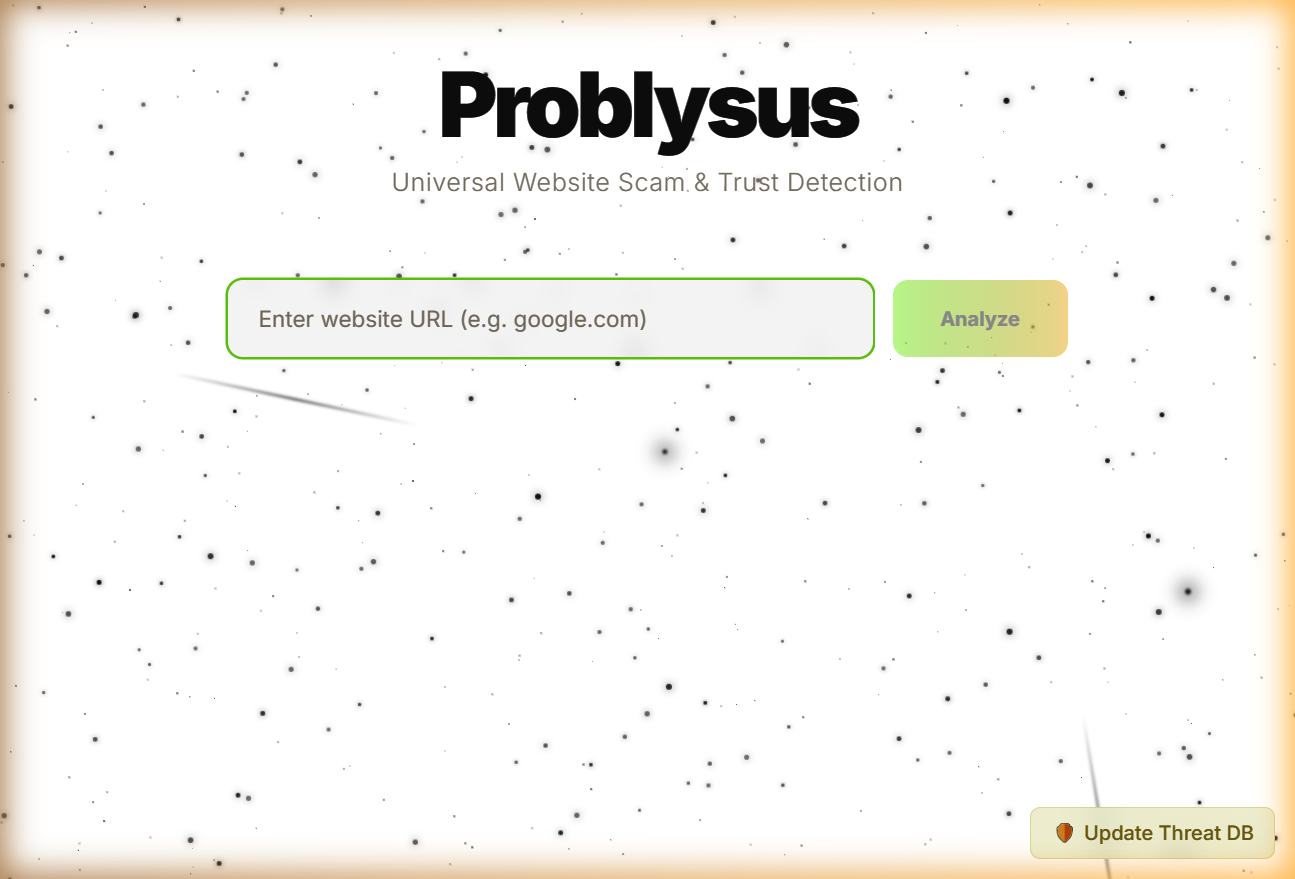
\includegraphics[width=0.85\textwidth]{images/chapter6/web_home_url_input.png}
\caption{Web Application Home Page — URL Input Interface}
\label{fig:web_home}
\end{figure}

The following figure shows the web application's URL input page where analysis begins.

\subsection{Tailwind CSS v4}

Tailwind CSS v4 is used for styling through utility classes. Its just-in-time compilation ensures minimal CSS bundle size and efficient rendering.

\subsection{Framer Motion}

Framer Motion provides UI animations such as fade-in panel transitions and animated privacy exposure bars.

\begin{figure}[!htbp]
\centering
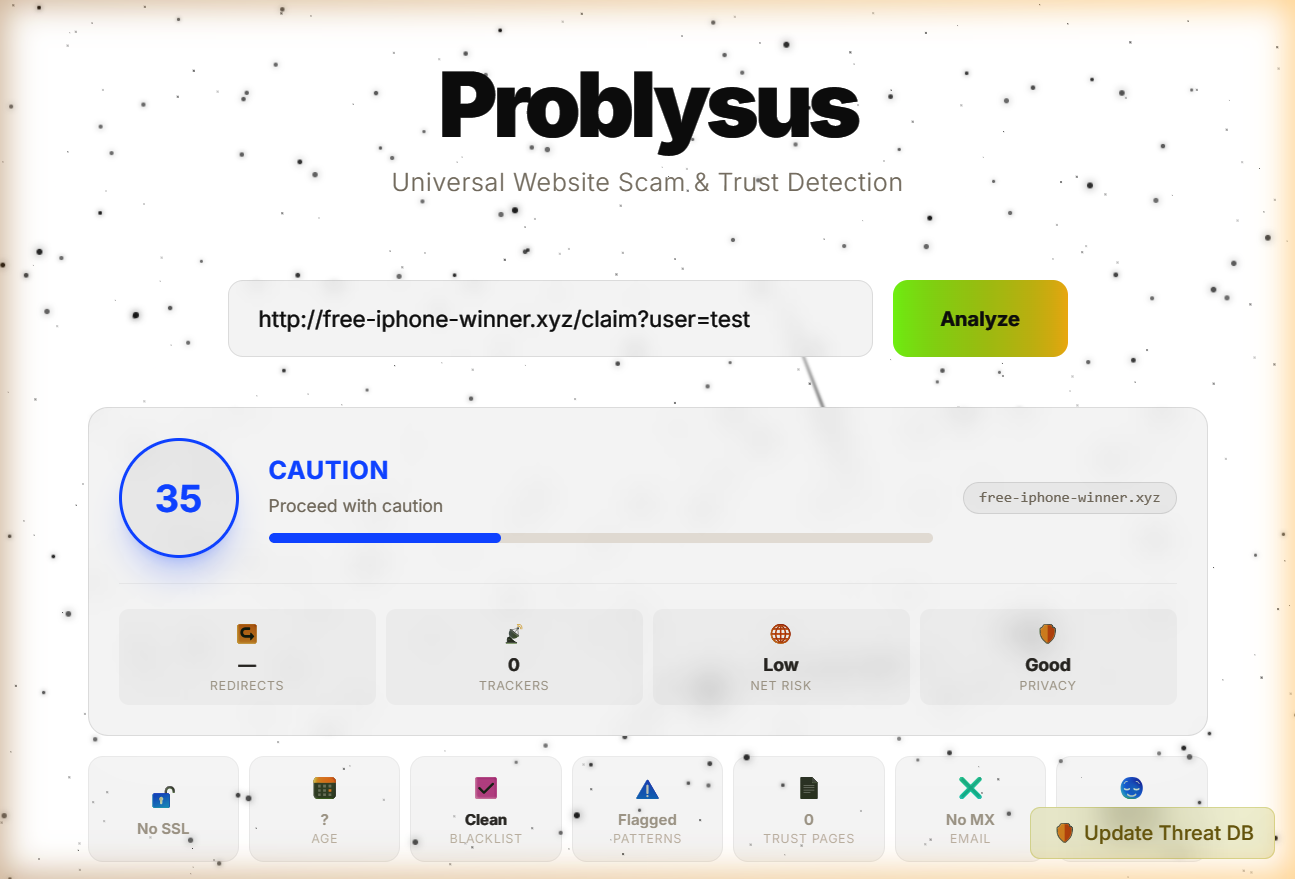
\includegraphics[width=0.85\textwidth]{images/chapter6/dashboard_panels.png}
\caption{Analysis Result Dashboard with Animated Panels}
\label{fig:dashboard_panels}
\end{figure}

The following figure demonstrates the dashboard layout used to present scan outputs.

\subsection{Axios}

Axios handles all HTTP communication between the React frontend and the Flask backend by sending POST requests to the analysis endpoint and receiving structured JSON responses.

\section{Backend Technologies}

\subsection{Python 3 / Flask}

The backend API is developed using Python 3 and the Flask micro-framework. Flask-CORS allows cross-origin requests from the React frontend and browser extension.

\begin{figure}[!htbp]
\centering
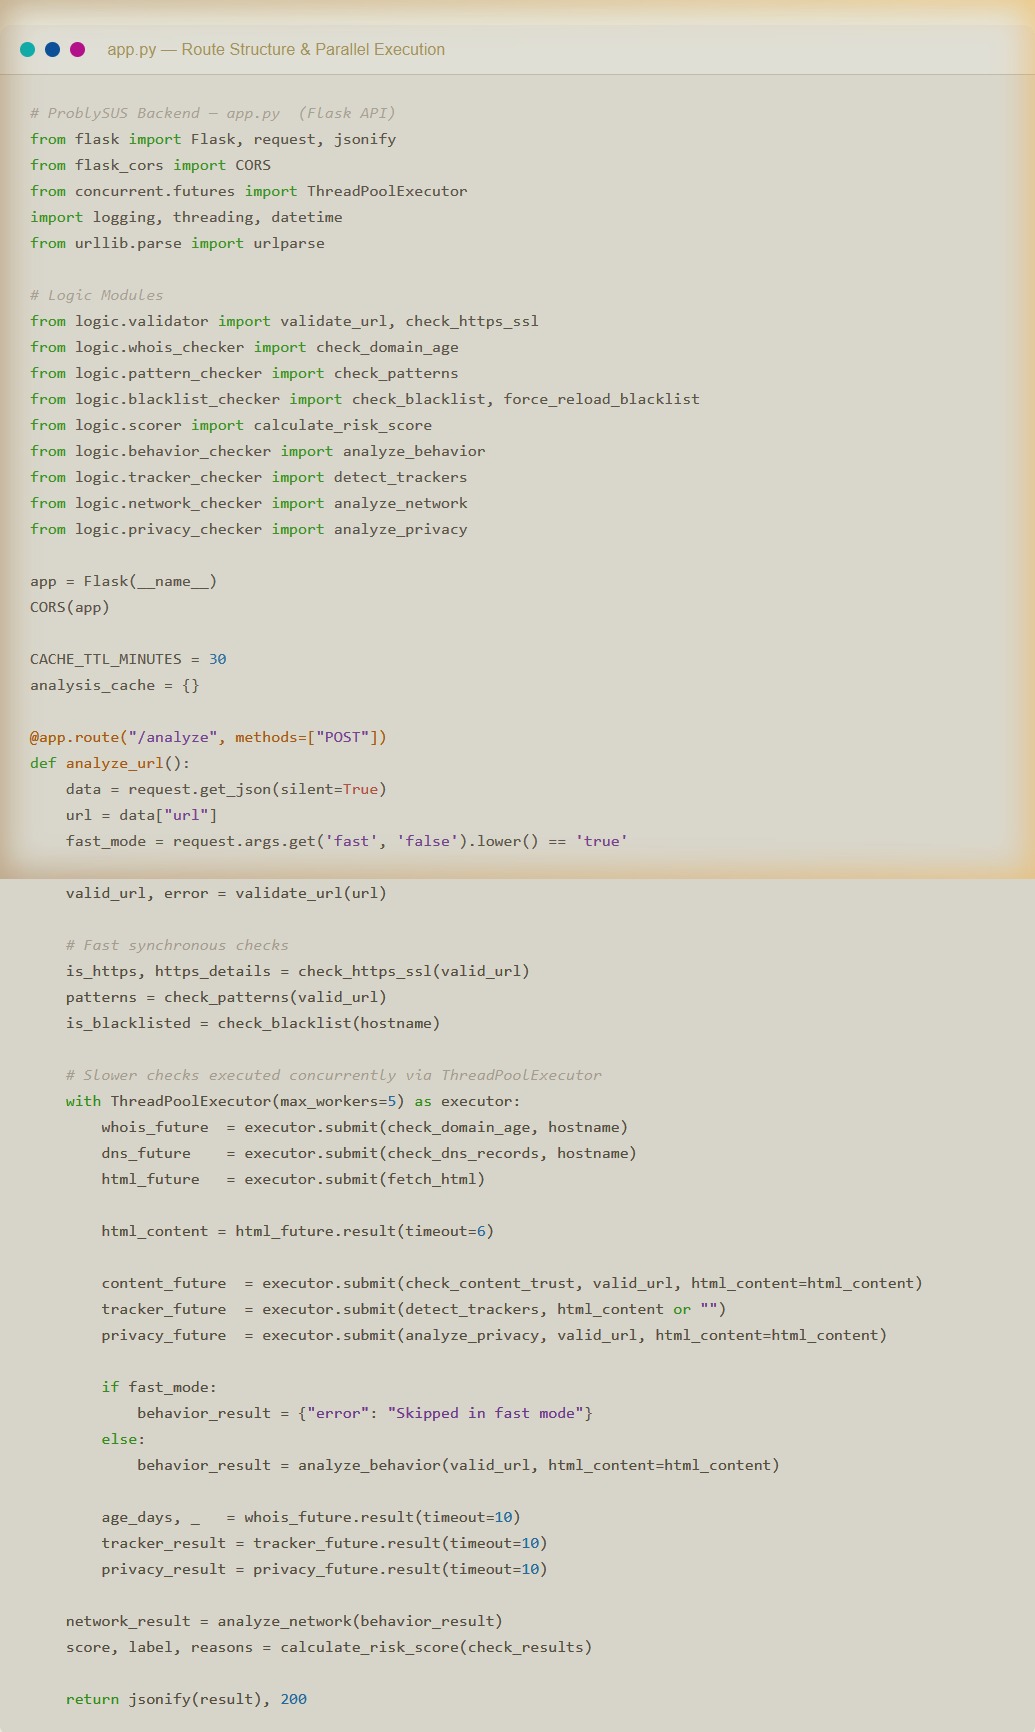
\includegraphics[width=0.8\textwidth]{images/chapter6/flask_routes.png}
\caption{Flask app.py Route Definitions and ThreadPoolExecutor Block}
\label{fig:flask_routes}
\end{figure}

\subsection{Concurrent Execution — ThreadPoolExecutor}

Python's \texttt{ThreadPoolExecutor} enables concurrent execution of network-dependent modules such as WHOIS lookup, DNS queries, and content analysis, reducing total processing time.

\subsection{Playwright + Chromium}

Playwright is used to launch a headless Chromium browser to simulate real browsing behavior and capture redirects and external requests.

\begin{figure}[!htbp]
\centering
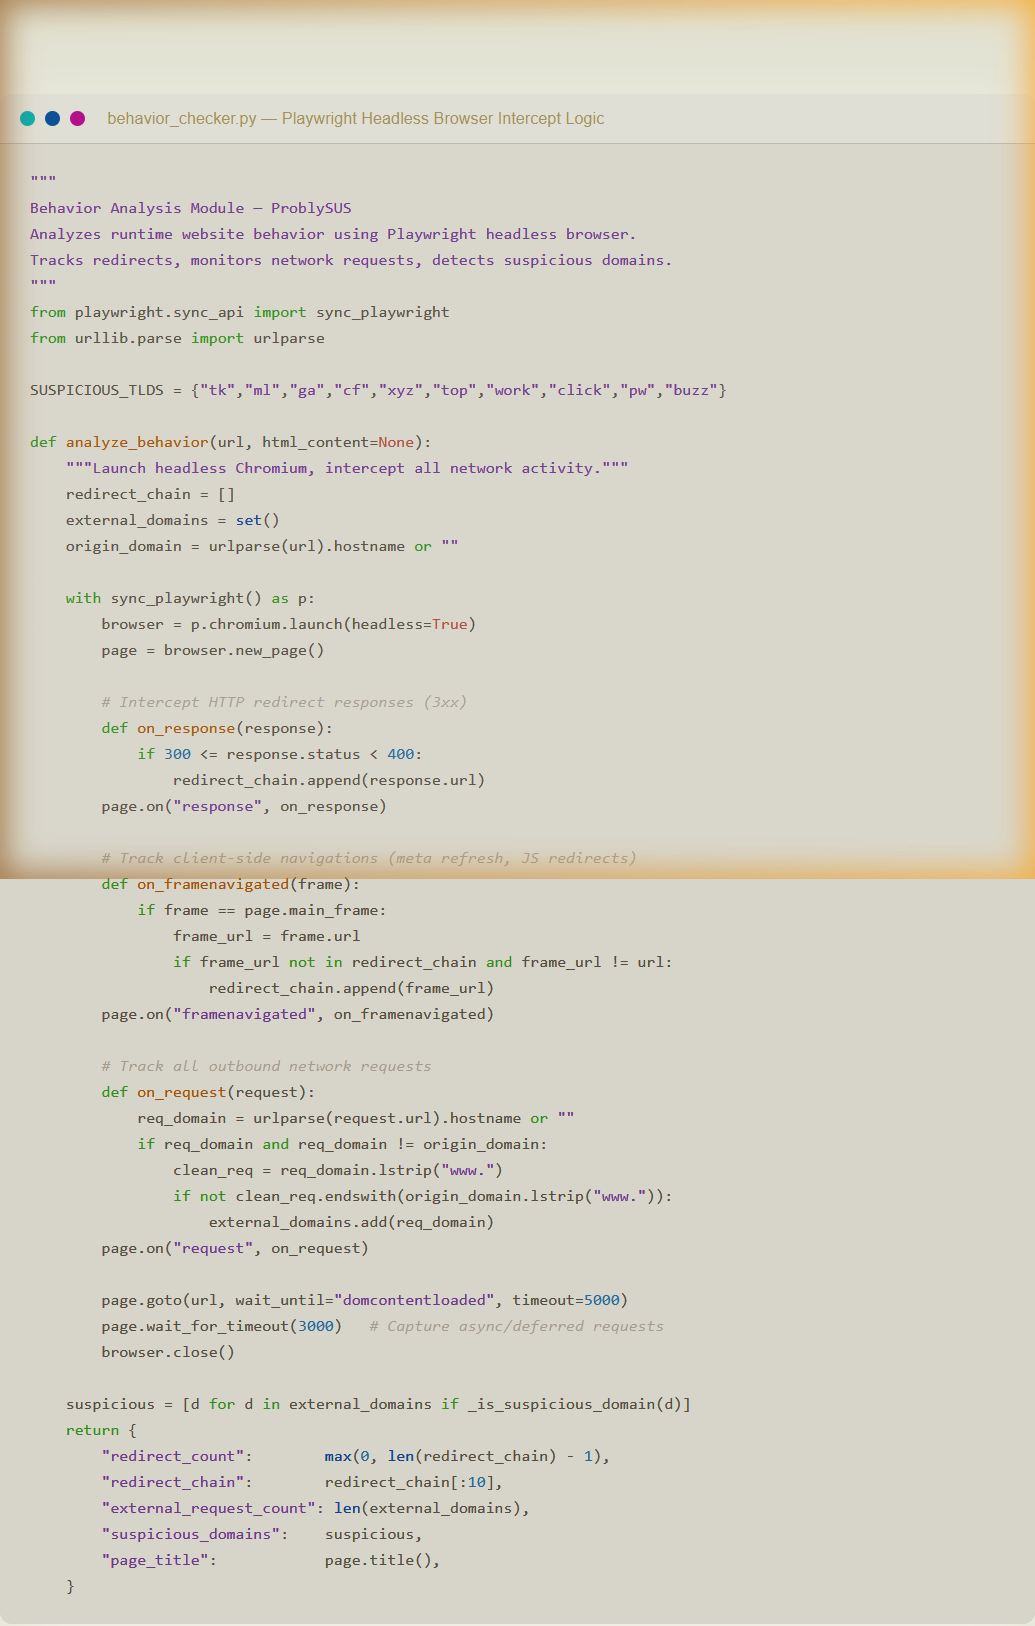
\includegraphics[width=0.8\textwidth]{images/chapter6/playwright_logic.png}
\caption{Playwright Launch and Network Interception Logic}
\label{fig:playwright_logic}
\end{figure}

\subsection{Analysis Libraries}

\begin{table}[h]
\centering
\begin{tabular}{|ll|}
\toprule
Library & Purpose \\
\midrule
requests & HTTP requests and feed downloads \\
python-whois & Domain registration queries \\
dnspython & DNS lookups for MX and SPF records \\
beautifulsoup4 & HTML parsing for analysis modules \\
tldextract & Domain extraction from URLs \\
textstat & Content readability scoring \\
re & Regular expression matching \\
csv / zipfile & URLhaus feed extraction \\
\bottomrule
\end{tabular}
\caption{Backend Analysis Libraries}
\end{table}

\section{Browser Extension Technologies}

The browser extension is built using Manifest V3 and plain HTML, CSS, and JavaScript for the popup interface.

\begin{figure}[!htbp]
\centering
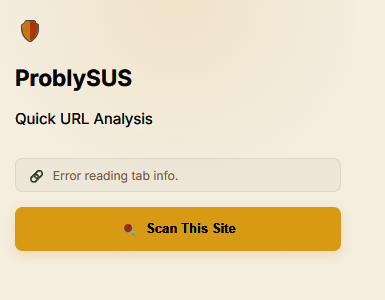
\includegraphics[width=0.75\textwidth]{images/chapter6/extension_overview.png}
\caption{Chrome Extension Popup — Overview Tab}
\label{fig:extension_overview}
\end{figure}

The following figure shows the extension overview tab with compact risk information.

The score arc is implemented using CSS transforms and transitions.

\begin{figure}[!htbp]
\centering
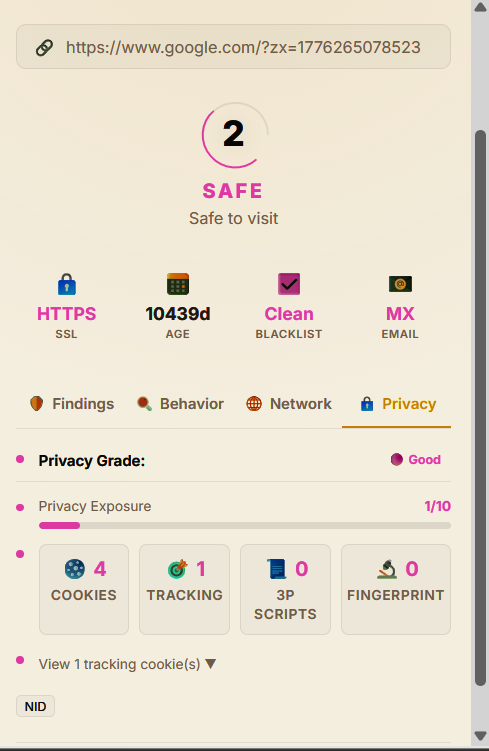
\includegraphics[width=0.75\textwidth]{images/chapter6/extension_privacy_tab.png}
\caption{Chrome Extension Popup — Behavior and Privacy Tabs}
\label{fig:extension_privacy_tab}
\end{figure}

The following figure shows behavior and privacy tabs for deeper inspection inside the extension.

\section{Threat Intelligence Tools}

\subsection{URLhaus Feed}

URLhaus provides a community-maintained dataset of malicious URLs distributed as a ZIP-compressed CSV feed.

\begin{figure}[!htbp]
\centering
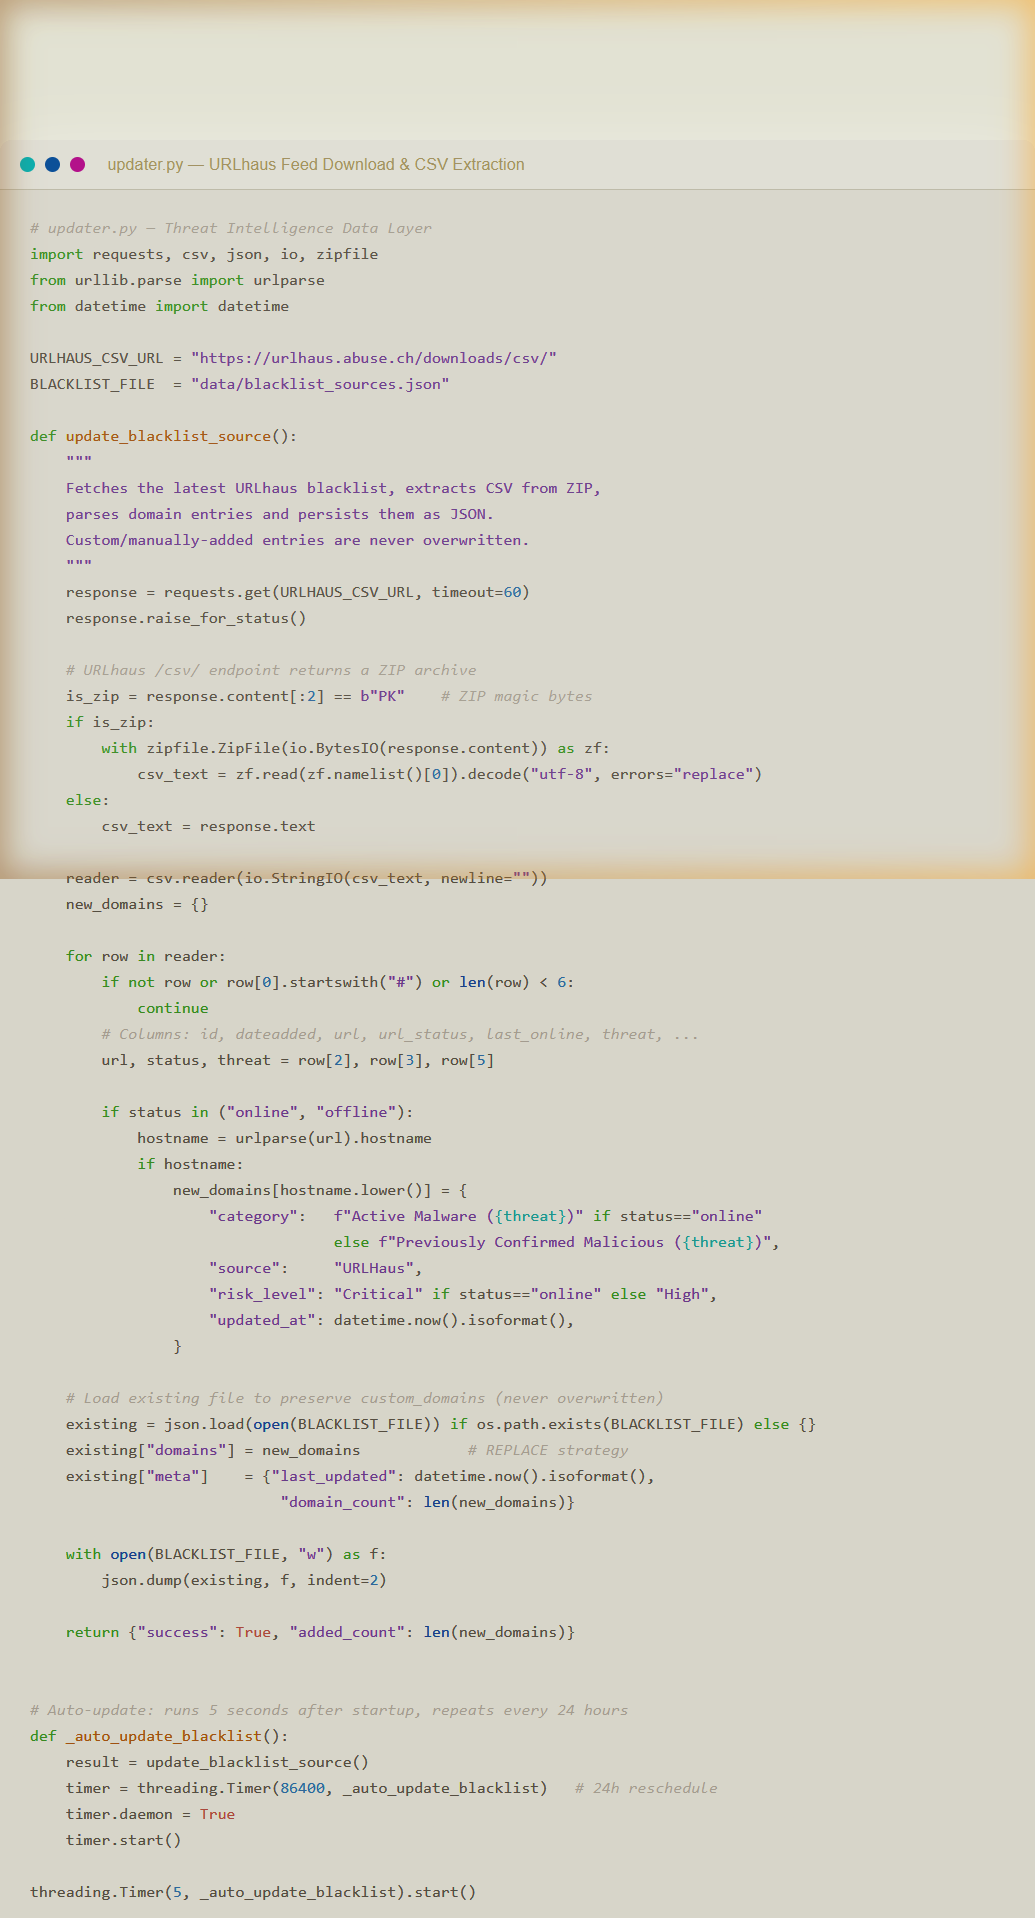
\includegraphics[width=0.75\textwidth]{images/chapter6/urlhaus_updater_logic.png}
\caption{URLhaus Feed Download and Auto-Refresh Logic}
\label{fig:urlhaus_updater}
\end{figure}

\subsection{Local Tracker Database}

A local \texttt{trackers.json} file maps known tracker domains to human-readable tracker names used during tracker detection.

\section{Testing Tools}

Postman was used for API endpoint testing, while Chrome DevTools was used for debugging frontend components and browser extension behavior. A custom \texttt{test\_scorer.py} script was used to unit-test the scoring engine independently.

\section{Version Control and Project Management}

Git was used for version control with a GitHub repository serving as the central codebase. The repository contains the full source tree including \texttt{backend/}, \texttt{frontend/}, \texttt{extension/}, and documentation files.

\section{Deployment}

ProblySUS currently runs locally with the Flask backend hosted at \texttt{http://127.0.0.1:5000} and the Vite frontend at \texttt{http://localhost:5173}. The Chrome extension is loaded as an unpacked extension via developer mode.

\section{Security Considerations}

Several security safeguards are implemented since the system analyzes potentially malicious URLs.

\begin{figure}[!htbp]
\centering
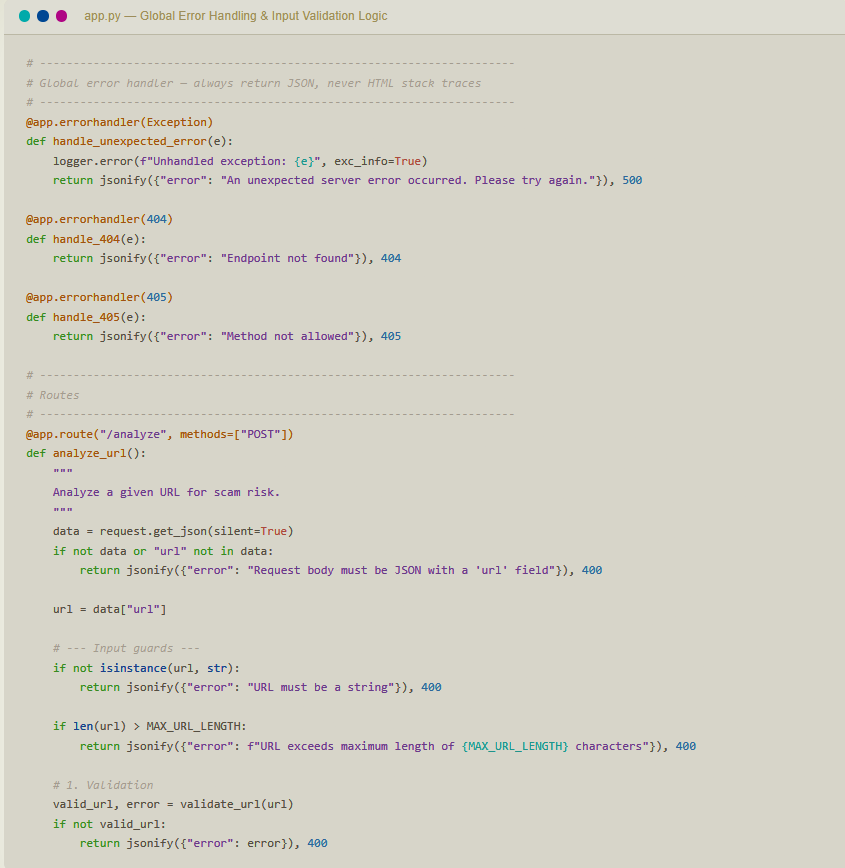
\includegraphics[width=0.8\textwidth]{images/chapter6/error_handler_validation.png}
\caption{Global Error Handling and Input Validation Logic in app.py}
\label{fig:error_handler}
\end{figure}

Playwright runs in a sandboxed environment and does not persist cookies between scans. All user input is validated before analysis, and error responses always return JSON to avoid exposing internal server details.
